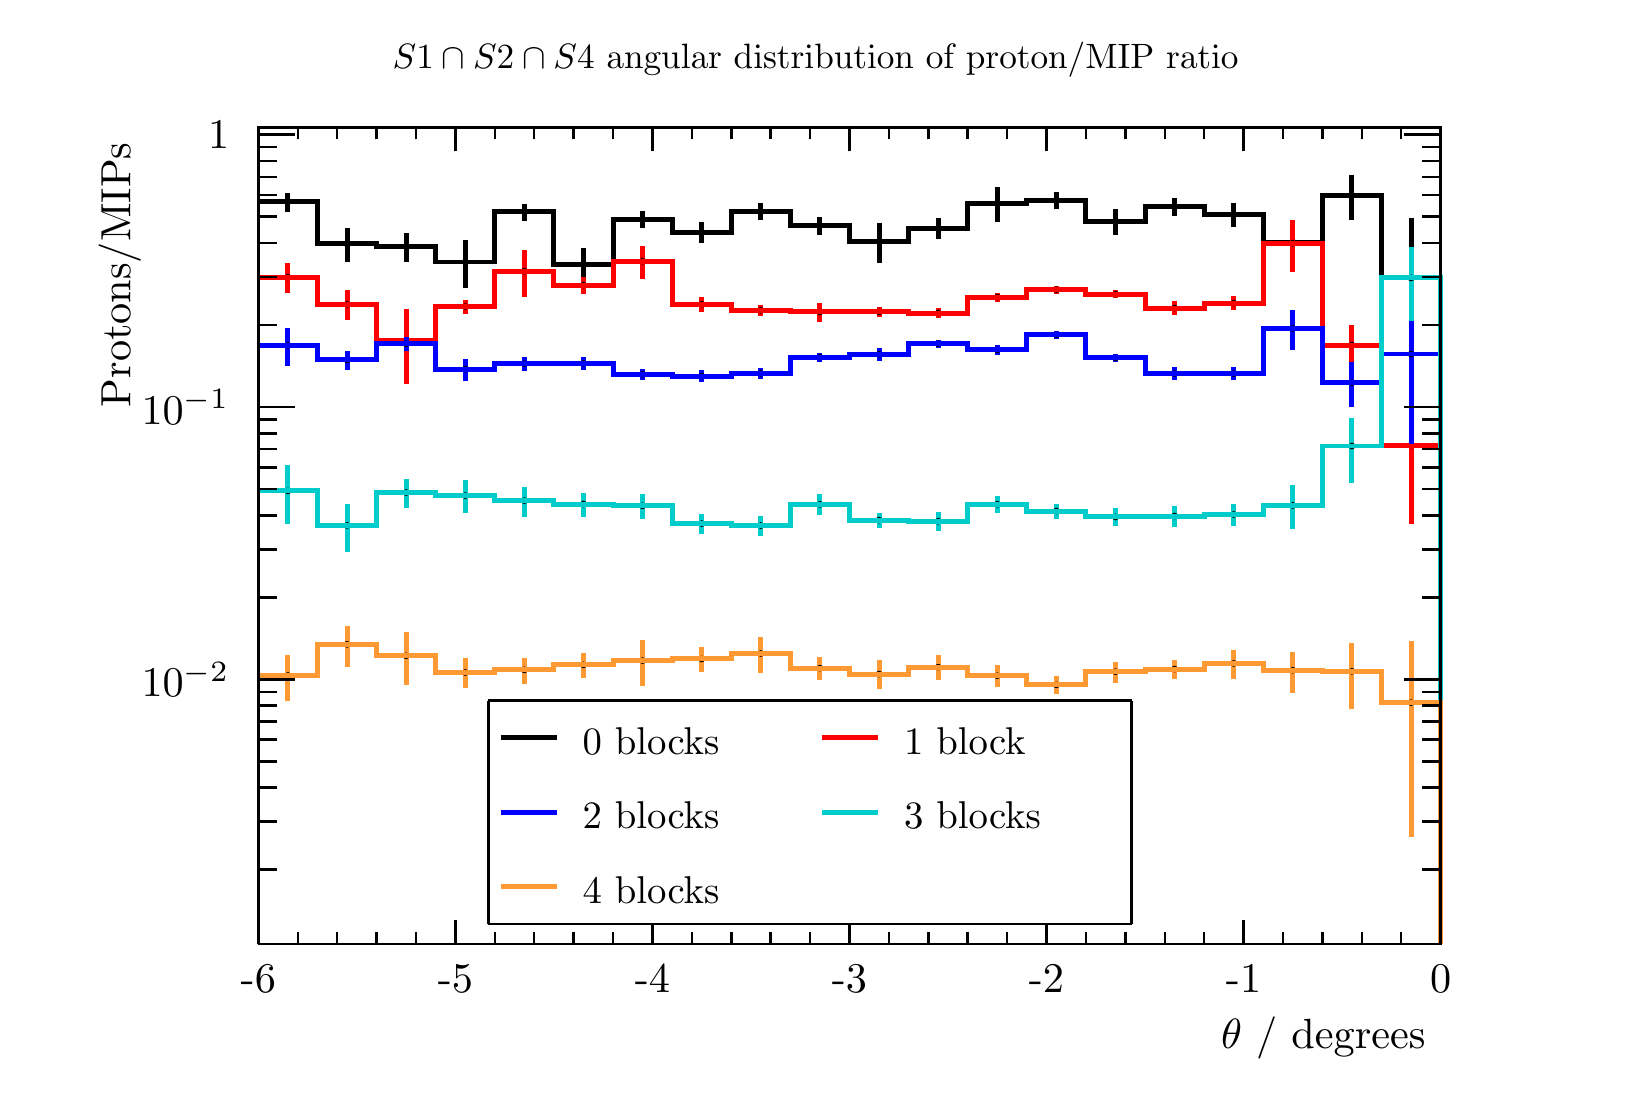
\begin{tikzpicture}
\pgfdeclareplotmark{cross} {
\pgfpathmoveto{\pgfpoint{-0.3\pgfplotmarksize}{\pgfplotmarksize}}
\pgfpathlineto{\pgfpoint{+0.3\pgfplotmarksize}{\pgfplotmarksize}}
\pgfpathlineto{\pgfpoint{+0.3\pgfplotmarksize}{0.3\pgfplotmarksize}}
\pgfpathlineto{\pgfpoint{+1\pgfplotmarksize}{0.3\pgfplotmarksize}}
\pgfpathlineto{\pgfpoint{+1\pgfplotmarksize}{-0.3\pgfplotmarksize}}
\pgfpathlineto{\pgfpoint{+0.3\pgfplotmarksize}{-0.3\pgfplotmarksize}}
\pgfpathlineto{\pgfpoint{+0.3\pgfplotmarksize}{-1.\pgfplotmarksize}}
\pgfpathlineto{\pgfpoint{-0.3\pgfplotmarksize}{-1.\pgfplotmarksize}}
\pgfpathlineto{\pgfpoint{-0.3\pgfplotmarksize}{-0.3\pgfplotmarksize}}
\pgfpathlineto{\pgfpoint{-1.\pgfplotmarksize}{-0.3\pgfplotmarksize}}
\pgfpathlineto{\pgfpoint{-1.\pgfplotmarksize}{0.3\pgfplotmarksize}}
\pgfpathlineto{\pgfpoint{-0.3\pgfplotmarksize}{0.3\pgfplotmarksize}}
\pgfpathclose
\pgfusepathqstroke
}
\pgfdeclareplotmark{cross*} {
\pgfpathmoveto{\pgfpoint{-0.3\pgfplotmarksize}{\pgfplotmarksize}}
\pgfpathlineto{\pgfpoint{+0.3\pgfplotmarksize}{\pgfplotmarksize}}
\pgfpathlineto{\pgfpoint{+0.3\pgfplotmarksize}{0.3\pgfplotmarksize}}
\pgfpathlineto{\pgfpoint{+1\pgfplotmarksize}{0.3\pgfplotmarksize}}
\pgfpathlineto{\pgfpoint{+1\pgfplotmarksize}{-0.3\pgfplotmarksize}}
\pgfpathlineto{\pgfpoint{+0.3\pgfplotmarksize}{-0.3\pgfplotmarksize}}
\pgfpathlineto{\pgfpoint{+0.3\pgfplotmarksize}{-1.\pgfplotmarksize}}
\pgfpathlineto{\pgfpoint{-0.3\pgfplotmarksize}{-1.\pgfplotmarksize}}
\pgfpathlineto{\pgfpoint{-0.3\pgfplotmarksize}{-0.3\pgfplotmarksize}}
\pgfpathlineto{\pgfpoint{-1.\pgfplotmarksize}{-0.3\pgfplotmarksize}}
\pgfpathlineto{\pgfpoint{-1.\pgfplotmarksize}{0.3\pgfplotmarksize}}
\pgfpathlineto{\pgfpoint{-0.3\pgfplotmarksize}{0.3\pgfplotmarksize}}
\pgfpathclose
\pgfusepathqfillstroke
}
\pgfdeclareplotmark{newstar} {
\pgfpathmoveto{\pgfqpoint{0pt}{\pgfplotmarksize}}
\pgfpathlineto{\pgfqpointpolar{44}{0.5\pgfplotmarksize}}
\pgfpathlineto{\pgfqpointpolar{18}{\pgfplotmarksize}}
\pgfpathlineto{\pgfqpointpolar{-20}{0.5\pgfplotmarksize}}
\pgfpathlineto{\pgfqpointpolar{-54}{\pgfplotmarksize}}
\pgfpathlineto{\pgfqpointpolar{-90}{0.5\pgfplotmarksize}}
\pgfpathlineto{\pgfqpointpolar{234}{\pgfplotmarksize}}
\pgfpathlineto{\pgfqpointpolar{198}{0.5\pgfplotmarksize}}
\pgfpathlineto{\pgfqpointpolar{162}{\pgfplotmarksize}}
\pgfpathlineto{\pgfqpointpolar{134}{0.5\pgfplotmarksize}}
\pgfpathclose
\pgfusepathqstroke
}
\pgfdeclareplotmark{newstar*} {
\pgfpathmoveto{\pgfqpoint{0pt}{\pgfplotmarksize}}
\pgfpathlineto{\pgfqpointpolar{44}{0.5\pgfplotmarksize}}
\pgfpathlineto{\pgfqpointpolar{18}{\pgfplotmarksize}}
\pgfpathlineto{\pgfqpointpolar{-20}{0.5\pgfplotmarksize}}
\pgfpathlineto{\pgfqpointpolar{-54}{\pgfplotmarksize}}
\pgfpathlineto{\pgfqpointpolar{-90}{0.5\pgfplotmarksize}}
\pgfpathlineto{\pgfqpointpolar{234}{\pgfplotmarksize}}
\pgfpathlineto{\pgfqpointpolar{198}{0.5\pgfplotmarksize}}
\pgfpathlineto{\pgfqpointpolar{162}{\pgfplotmarksize}}
\pgfpathlineto{\pgfqpointpolar{134}{0.5\pgfplotmarksize}}
\pgfpathclose
\pgfusepathqfillstroke
}
\definecolor{c}{rgb}{1,1,1};
\draw [color=c, fill=c] (0,0) rectangle (20,13.4957);
\draw [color=c, fill=c] (2.92264,1.86246) rectangle (17.937,12.235);
\definecolor{c}{rgb}{0,0,0};
\draw [c,line width=0.9] (2.92264,1.86246) -- (2.92264,12.235) -- (17.937,12.235) -- (17.937,1.86246) -- (2.92264,1.86246);
\definecolor{c}{rgb}{1,1,1};
\draw [color=c, fill=c] (2.92264,1.86246) rectangle (17.937,12.235);
\definecolor{c}{rgb}{0,0,0};
\draw [c,line width=0.9] (2.92264,1.86246) -- (2.92264,12.235) -- (17.937,12.235) -- (17.937,1.86246) -- (2.92264,1.86246);
\draw [c,line width=0.9] (2.92264,1.86246) -- (3.67335,1.86246) -- (3.67335,1.86246) -- (4.42407,1.86246) -- (4.42407,1.86246) -- (5.17479,1.86246) -- (5.17479,1.86246) -- (5.9255,1.86246) -- (5.9255,1.86246) -- (6.67622,1.86246) -- (6.67622,1.86246)
 -- (7.42693,1.86246) -- (7.42693,1.86246) -- (8.17765,1.86246) -- (8.17765,1.86246) -- (8.92837,1.86246) -- (8.92837,1.86246) -- (9.67908,1.86246) -- (9.67908,1.86246) -- (10.4298,1.86246) -- (10.4298,1.86246) -- (11.1805,1.86246) --
 (11.1805,1.86246) -- (11.9312,1.86246) -- (11.9312,1.86246) -- (12.6819,1.86246) -- (12.6819,1.86246) -- (13.4327,1.86246) -- (13.4327,1.86246) -- (14.1834,1.86246) -- (14.1834,1.86246) -- (14.9341,1.86246) -- (14.9341,1.86246) -- (15.6848,1.86246)
 -- (15.6848,1.86246) -- (16.4355,1.86246) -- (16.4355,1.86246) -- (17.1862,1.86246) -- (17.1862,1.86246) -- (17.937,1.86246) -- (17.937,1.86246);
\draw [c,line width=0.9] (2.92264,1.86246) -- (17.937,1.86246);
\draw [c,line width=0.9] (2.92264,2.16641) -- (2.92264,1.86246);
\draw [c,line width=0.9] (3.42311,2.01444) -- (3.42311,1.86246);
\draw [c,line width=0.9] (3.92359,2.01444) -- (3.92359,1.86246);
\draw [c,line width=0.9] (4.42407,2.01444) -- (4.42407,1.86246);
\draw [c,line width=0.9] (4.92455,2.01444) -- (4.92455,1.86246);
\draw [c,line width=0.9] (5.42502,2.16641) -- (5.42502,1.86246);
\draw [c,line width=0.9] (5.9255,2.01444) -- (5.9255,1.86246);
\draw [c,line width=0.9] (6.42598,2.01444) -- (6.42598,1.86246);
\draw [c,line width=0.9] (6.92646,2.01444) -- (6.92646,1.86246);
\draw [c,line width=0.9] (7.42693,2.01444) -- (7.42693,1.86246);
\draw [c,line width=0.9] (7.92741,2.16641) -- (7.92741,1.86246);
\draw [c,line width=0.9] (8.42789,2.01444) -- (8.42789,1.86246);
\draw [c,line width=0.9] (8.92837,2.01444) -- (8.92837,1.86246);
\draw [c,line width=0.9] (9.42884,2.01444) -- (9.42884,1.86246);
\draw [c,line width=0.9] (9.92932,2.01444) -- (9.92932,1.86246);
\draw [c,line width=0.9] (10.4298,2.16641) -- (10.4298,1.86246);
\draw [c,line width=0.9] (10.9303,2.01444) -- (10.9303,1.86246);
\draw [c,line width=0.9] (11.4308,2.01444) -- (11.4308,1.86246);
\draw [c,line width=0.9] (11.9312,2.01444) -- (11.9312,1.86246);
\draw [c,line width=0.9] (12.4317,2.01444) -- (12.4317,1.86246);
\draw [c,line width=0.9] (12.9322,2.16641) -- (12.9322,1.86246);
\draw [c,line width=0.9] (13.4327,2.01444) -- (13.4327,1.86246);
\draw [c,line width=0.9] (13.9331,2.01444) -- (13.9331,1.86246);
\draw [c,line width=0.9] (14.4336,2.01444) -- (14.4336,1.86246);
\draw [c,line width=0.9] (14.9341,2.01444) -- (14.9341,1.86246);
\draw [c,line width=0.9] (15.4346,2.16641) -- (15.4346,1.86246);
\draw [c,line width=0.9] (15.9351,2.01444) -- (15.9351,1.86246);
\draw [c,line width=0.9] (16.4355,2.01444) -- (16.4355,1.86246);
\draw [c,line width=0.9] (16.936,2.01444) -- (16.936,1.86246);
\draw [c,line width=0.9] (17.4365,2.01444) -- (17.4365,1.86246);
\draw [c,line width=0.9] (17.937,2.16641) -- (17.937,1.86246);
\draw [anchor=base] (2.92264,1.25516) node[scale=1.52731, color=c, rotate=0]{-6};
\draw [anchor=base] (5.42502,1.25516) node[scale=1.52731, color=c, rotate=0]{-5};
\draw [anchor=base] (7.92741,1.25516) node[scale=1.52731, color=c, rotate=0]{-4};
\draw [anchor=base] (10.4298,1.25516) node[scale=1.52731, color=c, rotate=0]{-3};
\draw [anchor=base] (12.9322,1.25516) node[scale=1.52731, color=c, rotate=0]{-2};
\draw [anchor=base] (15.4346,1.25516) node[scale=1.52731, color=c, rotate=0]{-1};
\draw [anchor=base] (17.937,1.25516) node[scale=1.52731, color=c, rotate=0]{0};
\draw [anchor= east] (17.937,0.674842) node[scale=1.52731, color=c, rotate=0]{$ \theta$ / degrees};
\draw [c,line width=0.9] (2.92264,12.235) -- (17.937,12.235);
\draw [c,line width=0.9] (2.92264,11.931) -- (2.92264,12.235);
\draw [c,line width=0.9] (3.42311,12.083) -- (3.42311,12.235);
\draw [c,line width=0.9] (3.92359,12.083) -- (3.92359,12.235);
\draw [c,line width=0.9] (4.42407,12.083) -- (4.42407,12.235);
\draw [c,line width=0.9] (4.92455,12.083) -- (4.92455,12.235);
\draw [c,line width=0.9] (5.42502,11.931) -- (5.42502,12.235);
\draw [c,line width=0.9] (5.9255,12.083) -- (5.9255,12.235);
\draw [c,line width=0.9] (6.42598,12.083) -- (6.42598,12.235);
\draw [c,line width=0.9] (6.92646,12.083) -- (6.92646,12.235);
\draw [c,line width=0.9] (7.42693,12.083) -- (7.42693,12.235);
\draw [c,line width=0.9] (7.92741,11.931) -- (7.92741,12.235);
\draw [c,line width=0.9] (8.42789,12.083) -- (8.42789,12.235);
\draw [c,line width=0.9] (8.92837,12.083) -- (8.92837,12.235);
\draw [c,line width=0.9] (9.42884,12.083) -- (9.42884,12.235);
\draw [c,line width=0.9] (9.92932,12.083) -- (9.92932,12.235);
\draw [c,line width=0.9] (10.4298,11.931) -- (10.4298,12.235);
\draw [c,line width=0.9] (10.9303,12.083) -- (10.9303,12.235);
\draw [c,line width=0.9] (11.4308,12.083) -- (11.4308,12.235);
\draw [c,line width=0.9] (11.9312,12.083) -- (11.9312,12.235);
\draw [c,line width=0.9] (12.4317,12.083) -- (12.4317,12.235);
\draw [c,line width=0.9] (12.9322,11.931) -- (12.9322,12.235);
\draw [c,line width=0.9] (13.4327,12.083) -- (13.4327,12.235);
\draw [c,line width=0.9] (13.9331,12.083) -- (13.9331,12.235);
\draw [c,line width=0.9] (14.4336,12.083) -- (14.4336,12.235);
\draw [c,line width=0.9] (14.9341,12.083) -- (14.9341,12.235);
\draw [c,line width=0.9] (15.4346,11.931) -- (15.4346,12.235);
\draw [c,line width=0.9] (15.9351,12.083) -- (15.9351,12.235);
\draw [c,line width=0.9] (16.4355,12.083) -- (16.4355,12.235);
\draw [c,line width=0.9] (16.936,12.083) -- (16.936,12.235);
\draw [c,line width=0.9] (17.4365,12.083) -- (17.4365,12.235);
\draw [c,line width=0.9] (17.937,11.931) -- (17.937,12.235);
\draw [c,line width=0.9] (2.92264,1.86246) -- (2.92264,12.235);
\draw [c,line width=0.9] (3.15321,2.80967) -- (2.92264,2.80967);
\draw [c,line width=0.9] (3.15321,3.41867) -- (2.92264,3.41867);
\draw [c,line width=0.9] (3.15321,3.85076) -- (2.92264,3.85076);
\draw [c,line width=0.9] (3.15321,4.18592) -- (2.92264,4.18592);
\draw [c,line width=0.9] (3.15321,4.45976) -- (2.92264,4.45976);
\draw [c,line width=0.9] (3.15321,4.69129) -- (2.92264,4.69129);
\draw [c,line width=0.9] (3.15321,4.89185) -- (2.92264,4.89185);
\draw [c,line width=0.9] (3.15321,5.06876) -- (2.92264,5.06876);
\draw [c,line width=0.9] (3.38378,5.22701) -- (2.92264,5.22701);
\draw [anchor= east] (2.74264,5.22701) node[scale=1.52731, color=c, rotate=0]{$10^{-2}$};
\draw [c,line width=0.9] (3.15321,6.2681) -- (2.92264,6.2681);
\draw [c,line width=0.9] (3.15321,6.87711) -- (2.92264,6.87711);
\draw [c,line width=0.9] (3.15321,7.3092) -- (2.92264,7.3092);
\draw [c,line width=0.9] (3.15321,7.64436) -- (2.92264,7.64436);
\draw [c,line width=0.9] (3.15321,7.9182) -- (2.92264,7.9182);
\draw [c,line width=0.9] (3.15321,8.14973) -- (2.92264,8.14973);
\draw [c,line width=0.9] (3.15321,8.35029) -- (2.92264,8.35029);
\draw [c,line width=0.9] (3.15321,8.5272) -- (2.92264,8.5272);
\draw [c,line width=0.9] (3.38378,8.68545) -- (2.92264,8.68545);
\draw [anchor= east] (2.74264,8.68545) node[scale=1.52731, color=c, rotate=0]{$10^{-1}$};
\draw [c,line width=0.9] (3.15321,9.72654) -- (2.92264,9.72654);
\draw [c,line width=0.9] (3.15321,10.3355) -- (2.92264,10.3355);
\draw [c,line width=0.9] (3.15321,10.7676) -- (2.92264,10.7676);
\draw [c,line width=0.9] (3.15321,11.1028) -- (2.92264,11.1028);
\draw [c,line width=0.9] (3.15321,11.3766) -- (2.92264,11.3766);
\draw [c,line width=0.9] (3.15321,11.6082) -- (2.92264,11.6082);
\draw [c,line width=0.9] (3.15321,11.8087) -- (2.92264,11.8087);
\draw [c,line width=0.9] (3.15321,11.9856) -- (2.92264,11.9856);
\draw [c,line width=0.9] (3.38378,12.1439) -- (2.92264,12.1439);
\draw [anchor= east] (2.74264,12.1439) node[scale=1.52731, color=c, rotate=0]{1};
\draw [anchor= east] (1.16264,12.235) node[scale=1.52731, color=c, rotate=90]{ Protons/MIPs};
\draw [c,line width=0.9] (17.937,1.86246) -- (17.937,12.235);
\draw [c,line width=0.9] (17.7064,2.80967) -- (17.937,2.80967);
\draw [c,line width=0.9] (17.7064,3.41867) -- (17.937,3.41867);
\draw [c,line width=0.9] (17.7064,3.85076) -- (17.937,3.85076);
\draw [c,line width=0.9] (17.7064,4.18592) -- (17.937,4.18592);
\draw [c,line width=0.9] (17.7064,4.45976) -- (17.937,4.45976);
\draw [c,line width=0.9] (17.7064,4.69129) -- (17.937,4.69129);
\draw [c,line width=0.9] (17.7064,4.89185) -- (17.937,4.89185);
\draw [c,line width=0.9] (17.7064,5.06876) -- (17.937,5.06876);
\draw [c,line width=0.9] (17.4758,5.22701) -- (17.937,5.22701);
\draw [c,line width=0.9] (17.7064,6.2681) -- (17.937,6.2681);
\draw [c,line width=0.9] (17.7064,6.87711) -- (17.937,6.87711);
\draw [c,line width=0.9] (17.7064,7.3092) -- (17.937,7.3092);
\draw [c,line width=0.9] (17.7064,7.64436) -- (17.937,7.64436);
\draw [c,line width=0.9] (17.7064,7.9182) -- (17.937,7.9182);
\draw [c,line width=0.9] (17.7064,8.14973) -- (17.937,8.14973);
\draw [c,line width=0.9] (17.7064,8.35029) -- (17.937,8.35029);
\draw [c,line width=0.9] (17.7064,8.5272) -- (17.937,8.5272);
\draw [c,line width=0.9] (17.4758,8.68545) -- (17.937,8.68545);
\draw [c,line width=0.9] (17.7064,9.72654) -- (17.937,9.72654);
\draw [c,line width=0.9] (17.7064,10.3355) -- (17.937,10.3355);
\draw [c,line width=0.9] (17.7064,10.7676) -- (17.937,10.7676);
\draw [c,line width=0.9] (17.7064,11.1028) -- (17.937,11.1028);
\draw [c,line width=0.9] (17.7064,11.3766) -- (17.937,11.3766);
\draw [c,line width=0.9] (17.7064,11.6082) -- (17.937,11.6082);
\draw [c,line width=0.9] (17.7064,11.8087) -- (17.937,11.8087);
\draw [c,line width=0.9] (17.7064,11.9856) -- (17.937,11.9856);
\draw [c,line width=0.9] (17.4758,12.1439) -- (17.937,12.1439);
\draw [c,line width=1.8] (3.29799,11.1598) -- (3.29799,11.2895);
\draw [c,line width=1.8] (3.29799,11.2895) -- (3.29799,11.409);
\foreach \P in {(3.29799,11.2895)}{\draw[mark options={color=c,fill=c},mark size=2.402402pt,mark=*,mark size=1pt] plot coordinates {\P};}
\draw [c,line width=1.8] (4.04871,10.5276) -- (4.04871,10.7573);
\draw [c,line width=1.8] (4.04871,10.7573) -- (4.04871,10.9564);
\foreach \P in {(4.04871,10.7573)}{\draw[mark options={color=c,fill=c},mark size=2.402402pt,mark=*,mark size=1pt] plot coordinates {\P};}
\draw [c,line width=1.8] (4.79943,10.5328) -- (4.79943,10.7264);
\draw [c,line width=1.8] (4.79943,10.7264) -- (4.79943,10.8978);
\foreach \P in {(4.79943,10.7264)}{\draw[mark options={color=c,fill=c},mark size=2.402402pt,mark=*,mark size=1pt] plot coordinates {\P};}
\draw [c,line width=1.8] (5.55014,10.1927) -- (5.55014,10.5267);
\draw [c,line width=1.8] (5.55014,10.5267) -- (5.55014,10.7998);
\foreach \P in {(5.55014,10.5267)}{\draw[mark options={color=c,fill=c},mark size=2.402402pt,mark=*,mark size=1pt] plot coordinates {\P};}
\draw [c,line width=1.8] (6.30086,11.0473) -- (6.30086,11.1619);
\draw [c,line width=1.8] (6.30086,11.1619) -- (6.30086,11.2683);
\foreach \P in {(6.30086,11.1619)}{\draw[mark options={color=c,fill=c},mark size=2.402402pt,mark=*,mark size=1pt] plot coordinates {\P};}
\draw [c,line width=1.8] (7.05158,10.2689) -- (7.05158,10.4992);
\draw [c,line width=1.8] (7.05158,10.4992) -- (7.05158,10.6988);
\foreach \P in {(7.05158,10.4992)}{\draw[mark options={color=c,fill=c},mark size=2.402402pt,mark=*,mark size=1pt] plot coordinates {\P};}
\draw [c,line width=1.8] (7.80229,10.9523) -- (7.80229,11.0665);
\draw [c,line width=1.8] (7.80229,11.0665) -- (7.80229,11.1726);
\foreach \P in {(7.80229,11.0665)}{\draw[mark options={color=c,fill=c},mark size=2.402402pt,mark=*,mark size=1pt] plot coordinates {\P};}
\draw [c,line width=1.8] (8.55301,10.7721) -- (8.55301,10.9065);
\draw [c,line width=1.8] (8.55301,10.9065) -- (8.55301,11.0298);
\foreach \P in {(8.55301,10.9065)}{\draw[mark options={color=c,fill=c},mark size=2.402402pt,mark=*,mark size=1pt] plot coordinates {\P};}
\draw [c,line width=1.8] (9.30373,11.0554) -- (9.30373,11.1696);
\draw [c,line width=1.8] (9.30373,11.1696) -- (9.30373,11.2757);
\foreach \P in {(9.30373,11.1696)}{\draw[mark options={color=c,fill=c},mark size=2.402402pt,mark=*,mark size=1pt] plot coordinates {\P};}
\draw [c,line width=1.8] (10.0544,10.8699) -- (10.0544,10.99);
\draw [c,line width=1.8] (10.0544,10.99) -- (10.0544,11.1011);
\foreach \P in {(10.0544,10.99)}{\draw[mark options={color=c,fill=c},mark size=2.402402pt,mark=*,mark size=1pt] plot coordinates {\P};}
\draw [c,line width=1.8] (10.8052,10.5121) -- (10.8052,10.7855);
\draw [c,line width=1.8] (10.8052,10.7855) -- (10.8052,11.0167);
\foreach \P in {(10.8052,10.7855)}{\draw[mark options={color=c,fill=c},mark size=2.402402pt,mark=*,mark size=1pt] plot coordinates {\P};}
\draw [c,line width=1.8] (11.5559,10.8154) -- (11.5559,10.9531);
\draw [c,line width=1.8] (11.5559,10.9531) -- (11.5559,11.0793);
\foreach \P in {(11.5559,10.9531)}{\draw[mark options={color=c,fill=c},mark size=2.402402pt,mark=*,mark size=1pt] plot coordinates {\P};}
\draw [c,line width=1.8] (12.3066,11.0295) -- (12.3066,11.271);
\draw [c,line width=1.8] (12.3066,11.271) -- (12.3066,11.479);
\foreach \P in {(12.3066,11.271)}{\draw[mark options={color=c,fill=c},mark size=2.402402pt,mark=*,mark size=1pt] plot coordinates {\P};}
\draw [c,line width=1.8] (13.0573,11.1978) -- (13.0573,11.3121);
\draw [c,line width=1.8] (13.0573,11.3121) -- (13.0573,11.4183);
\foreach \P in {(13.0573,11.3121)}{\draw[mark options={color=c,fill=c},mark size=2.402402pt,mark=*,mark size=1pt] plot coordinates {\P};}
\draw [c,line width=1.8] (13.808,10.873) -- (13.808,11.0451);
\draw [c,line width=1.8] (13.808,11.0451) -- (13.808,11.1996);
\foreach \P in {(13.808,11.0451)}{\draw[mark options={color=c,fill=c},mark size=2.402402pt,mark=*,mark size=1pt] plot coordinates {\P};}
\draw [c,line width=1.8] (14.5587,11.1109) -- (14.5587,11.231);
\draw [c,line width=1.8] (14.5587,11.231) -- (14.5587,11.3423);
\foreach \P in {(14.5587,11.231)}{\draw[mark options={color=c,fill=c},mark size=2.402402pt,mark=*,mark size=1pt] plot coordinates {\P};}
\draw [c,line width=1.8] (15.3095,10.968) -- (15.3095,11.127);
\draw [c,line width=1.8] (15.3095,11.127) -- (15.3095,11.2709);
\foreach \P in {(15.3095,11.127)}{\draw[mark options={color=c,fill=c},mark size=2.402402pt,mark=*,mark size=1pt] plot coordinates {\P};}
\draw [c,line width=1.8] (16.0602,10.5735) -- (16.0602,10.7805);
\draw [c,line width=1.8] (16.0602,10.7805) -- (16.0602,10.9624);
\foreach \P in {(16.0602,10.7805)}{\draw[mark options={color=c,fill=c},mark size=2.402402pt,mark=*,mark size=1pt] plot coordinates {\P};}
\draw [c,line width=1.8] (16.8109,11.064) -- (16.8109,11.3741);
\draw [c,line width=1.8] (16.8109,11.3741) -- (16.8109,11.631);
\foreach \P in {(16.8109,11.3741)}{\draw[mark options={color=c,fill=c},mark size=2.402402pt,mark=*,mark size=1pt] plot coordinates {\P};}
\draw [c,line width=1.8] (17.5616,8.73957) -- (17.5616,10.3267);
\draw [c,line width=1.8] (17.5616,10.3267) -- (17.5616,11.081);
\foreach \P in {(17.5616,10.3267)}{\draw[mark options={color=c,fill=c},mark size=2.402402pt,mark=*,mark size=1pt] plot coordinates {\P};}
\draw [c,line width=1.8] (2.92264,11.2895) -- (3.67335,11.2895) -- (3.67335,10.7573) -- (4.42407,10.7573) -- (4.42407,10.7264) -- (5.17479,10.7264) -- (5.17479,10.5267) -- (5.9255,10.5267) -- (5.9255,11.1619) -- (6.67622,11.1619) -- (6.67622,10.4992)
 -- (7.42693,10.4992) -- (7.42693,11.0665) -- (8.17765,11.0665) -- (8.17765,10.9065) -- (8.92837,10.9065) -- (8.92837,11.1696) -- (9.67908,11.1696) -- (9.67908,10.99) -- (10.4298,10.99) -- (10.4298,10.7855) -- (11.1805,10.7855) -- (11.1805,10.9531)
 -- (11.9312,10.9531) -- (11.9312,11.271) -- (12.6819,11.271) -- (12.6819,11.3121) -- (13.4327,11.3121) -- (13.4327,11.0451) -- (14.1834,11.0451) -- (14.1834,11.231) -- (14.9341,11.231) -- (14.9341,11.127) -- (15.6848,11.127) -- (15.6848,10.7805) --
 (16.4355,10.7805) -- (16.4355,11.3741) -- (17.1862,11.3741) -- (17.1862,10.3267) -- (17.937,10.3267) -- (17.937,1.86246);
\definecolor{c}{rgb}{1,0,0};
\draw [c,line width=1.8] (3.29799,10.1299) -- (3.29799,10.3346);
\draw [c,line width=1.8] (3.29799,10.3346) -- (3.29799,10.5147);
\definecolor{c}{rgb}{0,0,0};
\foreach \P in {(3.29799,10.3346)}{\draw[mark options={color=c,fill=c},mark size=2.402402pt,mark=*,mark size=1pt] plot coordinates {\P};}
\definecolor{c}{rgb}{1,0,0};
\draw [c,line width=1.8] (4.04871,9.78499) -- (4.04871,9.98997);
\draw [c,line width=1.8] (4.04871,9.98997) -- (4.04871,10.1703);
\definecolor{c}{rgb}{0,0,0};
\foreach \P in {(4.04871,9.98997)}{\draw[mark options={color=c,fill=c},mark size=2.402402pt,mark=*,mark size=1pt] plot coordinates {\P};}
\definecolor{c}{rgb}{1,0,0};
\draw [c,line width=1.8] (4.79943,8.97546) -- (4.79943,9.52647);
\draw [c,line width=1.8] (4.79943,9.52647) -- (4.79943,9.92871);
\definecolor{c}{rgb}{0,0,0};
\foreach \P in {(4.79943,9.52647)}{\draw[mark options={color=c,fill=c},mark size=2.402402pt,mark=*,mark size=1pt] plot coordinates {\P};}
\definecolor{c}{rgb}{1,0,0};
\draw [c,line width=1.8] (5.55014,9.86977) -- (5.55014,9.9611);
\draw [c,line width=1.8] (5.55014,9.9611) -- (5.55014,10.0472);
\definecolor{c}{rgb}{0,0,0};
\foreach \P in {(5.55014,9.9611)}{\draw[mark options={color=c,fill=c},mark size=2.402402pt,mark=*,mark size=1pt] plot coordinates {\P};}
\definecolor{c}{rgb}{1,0,0};
\draw [c,line width=1.8] (6.30086,10.0823) -- (6.30086,10.4102);
\draw [c,line width=1.8] (6.30086,10.4102) -- (6.30086,10.6793);
\definecolor{c}{rgb}{0,0,0};
\foreach \P in {(6.30086,10.4102)}{\draw[mark options={color=c,fill=c},mark size=2.402402pt,mark=*,mark size=1pt] plot coordinates {\P};}
\definecolor{c}{rgb}{1,0,0};
\draw [c,line width=1.8] (7.05158,10.1166) -- (7.05158,10.2332);
\draw [c,line width=1.8] (7.05158,10.2332) -- (7.05158,10.3413);
\definecolor{c}{rgb}{0,0,0};
\foreach \P in {(7.05158,10.2332)}{\draw[mark options={color=c,fill=c},mark size=2.402402pt,mark=*,mark size=1pt] plot coordinates {\P};}
\definecolor{c}{rgb}{1,0,0};
\draw [c,line width=1.8] (7.80229,10.3061) -- (7.80229,10.536);
\draw [c,line width=1.8] (7.80229,10.536) -- (7.80229,10.7354);
\definecolor{c}{rgb}{0,0,0};
\foreach \P in {(7.80229,10.536)}{\draw[mark options={color=c,fill=c},mark size=2.402402pt,mark=*,mark size=1pt] plot coordinates {\P};}
\definecolor{c}{rgb}{1,0,0};
\draw [c,line width=1.8] (8.55301,9.89787) -- (8.55301,9.99034);
\draw [c,line width=1.8] (8.55301,9.99034) -- (8.55301,10.0774);
\definecolor{c}{rgb}{0,0,0};
\foreach \P in {(8.55301,9.99034)}{\draw[mark options={color=c,fill=c},mark size=2.402402pt,mark=*,mark size=1pt] plot coordinates {\P};}
\definecolor{c}{rgb}{1,0,0};
\draw [c,line width=1.8] (9.30373,9.84362) -- (9.30373,9.91308);
\draw [c,line width=1.8] (9.30373,9.91308) -- (9.30373,9.97947);
\definecolor{c}{rgb}{0,0,0};
\foreach \P in {(9.30373,9.91308)}{\draw[mark options={color=c,fill=c},mark size=2.402402pt,mark=*,mark size=1pt] plot coordinates {\P};}
\definecolor{c}{rgb}{1,0,0};
\draw [c,line width=1.8] (10.0544,9.76945) -- (10.0544,9.89208);
\draw [c,line width=1.8] (10.0544,9.89208) -- (10.0544,10.0055);
\definecolor{c}{rgb}{0,0,0};
\foreach \P in {(10.0544,9.89208)}{\draw[mark options={color=c,fill=c},mark size=2.402402pt,mark=*,mark size=1pt] plot coordinates {\P};}
\definecolor{c}{rgb}{1,0,0};
\draw [c,line width=1.8] (10.8052,9.82203) -- (10.8052,9.89281);
\draw [c,line width=1.8] (10.8052,9.89281) -- (10.8052,9.96039);
\definecolor{c}{rgb}{0,0,0};
\foreach \P in {(10.8052,9.89281)}{\draw[mark options={color=c,fill=c},mark size=2.402402pt,mark=*,mark size=1pt] plot coordinates {\P};}
\definecolor{c}{rgb}{1,0,0};
\draw [c,line width=1.8] (11.5559,9.81107) -- (11.5559,9.87836);
\draw [c,line width=1.8] (11.5559,9.87836) -- (11.5559,9.94277);
\definecolor{c}{rgb}{0,0,0};
\foreach \P in {(11.5559,9.87836)}{\draw[mark options={color=c,fill=c},mark size=2.402402pt,mark=*,mark size=1pt] plot coordinates {\P};}
\definecolor{c}{rgb}{1,0,0};
\draw [c,line width=1.8] (12.3066,10.0241) -- (12.3066,10.0799);
\draw [c,line width=1.8] (12.3066,10.0799) -- (12.3066,10.1337);
\definecolor{c}{rgb}{0,0,0};
\foreach \P in {(12.3066,10.0799)}{\draw[mark options={color=c,fill=c},mark size=2.402402pt,mark=*,mark size=1pt] plot coordinates {\P};}
\definecolor{c}{rgb}{1,0,0};
\draw [c,line width=1.8] (13.0573,10.1223) -- (13.0573,10.1759);
\draw [c,line width=1.8] (13.0573,10.1759) -- (13.0573,10.2276);
\definecolor{c}{rgb}{0,0,0};
\foreach \P in {(13.0573,10.1759)}{\draw[mark options={color=c,fill=c},mark size=2.402402pt,mark=*,mark size=1pt] plot coordinates {\P};}
\definecolor{c}{rgb}{1,0,0};
\draw [c,line width=1.8] (13.808,10.0649) -- (13.808,10.1174);
\draw [c,line width=1.8] (13.808,10.1174) -- (13.808,10.1681);
\definecolor{c}{rgb}{0,0,0};
\foreach \P in {(13.808,10.1174)}{\draw[mark options={color=c,fill=c},mark size=2.402402pt,mark=*,mark size=1pt] plot coordinates {\P};}
\definecolor{c}{rgb}{1,0,0};
\draw [c,line width=1.8] (14.5587,9.85252) -- (14.5587,9.94207);
\draw [c,line width=1.8] (14.5587,9.94207) -- (14.5587,10.0266);
\definecolor{c}{rgb}{0,0,0};
\foreach \P in {(14.5587,9.94207)}{\draw[mark options={color=c,fill=c},mark size=2.402402pt,mark=*,mark size=1pt] plot coordinates {\P};}
\definecolor{c}{rgb}{1,0,0};
\draw [c,line width=1.8] (15.3095,9.91085) -- (15.3095,10.0042);
\draw [c,line width=1.8] (15.3095,10.0042) -- (15.3095,10.0921);
\definecolor{c}{rgb}{0,0,0};
\foreach \P in {(15.3095,10.0042)}{\draw[mark options={color=c,fill=c},mark size=2.402402pt,mark=*,mark size=1pt] plot coordinates {\P};}
\definecolor{c}{rgb}{1,0,0};
\draw [c,line width=1.8] (16.0602,10.3948) -- (16.0602,10.7658);
\draw [c,line width=1.8] (16.0602,10.7658) -- (16.0602,11.0631);
\definecolor{c}{rgb}{0,0,0};
\foreach \P in {(16.0602,10.7658)}{\draw[mark options={color=c,fill=c},mark size=2.402402pt,mark=*,mark size=1pt] plot coordinates {\P};}
\definecolor{c}{rgb}{1,0,0};
\draw [c,line width=1.8] (16.8109,9.16401) -- (16.8109,9.4722);
\draw [c,line width=1.8] (16.8109,9.4722) -- (16.8109,9.72779);
\definecolor{c}{rgb}{0,0,0};
\foreach \P in {(16.8109,9.4722)}{\draw[mark options={color=c,fill=c},mark size=2.402402pt,mark=*,mark size=1pt] plot coordinates {\P};}
\definecolor{c}{rgb}{1,0,0};
\draw [c,line width=1.8] (17.5616,7.19654) -- (17.5616,8.20192);
\draw [c,line width=1.8] (17.5616,8.20192) -- (17.5616,8.79883);
\definecolor{c}{rgb}{0,0,0};
\foreach \P in {(17.5616,8.20192)}{\draw[mark options={color=c,fill=c},mark size=2.402402pt,mark=*,mark size=1pt] plot coordinates {\P};}
\definecolor{c}{rgb}{1,0,0};
\draw [c,line width=1.8] (2.92264,10.3346) -- (3.67335,10.3346) -- (3.67335,9.98997) -- (4.42407,9.98997) -- (4.42407,9.52647) -- (5.17479,9.52647) -- (5.17479,9.9611) -- (5.9255,9.9611) -- (5.9255,10.4102) -- (6.67622,10.4102) -- (6.67622,10.2332)
 -- (7.42693,10.2332) -- (7.42693,10.536) -- (8.17765,10.536) -- (8.17765,9.99034) -- (8.92837,9.99034) -- (8.92837,9.91308) -- (9.67908,9.91308) -- (9.67908,9.89208) -- (10.4298,9.89208) -- (10.4298,9.89281) -- (11.1805,9.89281) -- (11.1805,9.87836)
 -- (11.9312,9.87836) -- (11.9312,10.0799) -- (12.6819,10.0799) -- (12.6819,10.1759) -- (13.4327,10.1759) -- (13.4327,10.1174) -- (14.1834,10.1174) -- (14.1834,9.94207) -- (14.9341,9.94207) -- (14.9341,10.0042) -- (15.6848,10.0042) --
 (15.6848,10.7658) -- (16.4355,10.7658) -- (16.4355,9.4722) -- (17.1862,9.4722) -- (17.1862,8.20192) -- (17.937,8.20192) -- (17.937,1.86246);
\definecolor{c}{rgb}{0,0,1};
\draw [c,line width=1.8] (3.29799,9.20916) -- (3.29799,9.46699);
\draw [c,line width=1.8] (3.29799,9.46699) -- (3.29799,9.68697);
\definecolor{c}{rgb}{0,0,0};
\foreach \P in {(3.29799,9.46699)}{\draw[mark options={color=c,fill=c},mark size=2.402402pt,mark=*,mark size=1pt] plot coordinates {\P};}
\definecolor{c}{rgb}{0,0,1};
\draw [c,line width=1.8] (4.04871,9.15481) -- (4.04871,9.28329);
\draw [c,line width=1.8] (4.04871,9.28329) -- (4.04871,9.40165);
\definecolor{c}{rgb}{0,0,0};
\foreach \P in {(4.04871,9.28329)}{\draw[mark options={color=c,fill=c},mark size=2.402402pt,mark=*,mark size=1pt] plot coordinates {\P};}
\definecolor{c}{rgb}{0,0,1};
\draw [c,line width=1.8] (4.79943,9.39074) -- (4.79943,9.48774);
\draw [c,line width=1.8] (4.79943,9.48774) -- (4.79943,9.57885);
\definecolor{c}{rgb}{0,0,0};
\foreach \P in {(4.79943,9.48774)}{\draw[mark options={color=c,fill=c},mark size=2.402402pt,mark=*,mark size=1pt] plot coordinates {\P};}
\definecolor{c}{rgb}{0,0,1};
\draw [c,line width=1.8] (5.55014,9.01964) -- (5.55014,9.16496);
\draw [c,line width=1.8] (5.55014,9.16496) -- (5.55014,9.29744);
\definecolor{c}{rgb}{0,0,0};
\foreach \P in {(5.55014,9.16496)}{\draw[mark options={color=c,fill=c},mark size=2.402402pt,mark=*,mark size=1pt] plot coordinates {\P};}
\definecolor{c}{rgb}{0,0,1};
\draw [c,line width=1.8] (6.30086,9.14093) -- (6.30086,9.23629);
\draw [c,line width=1.8] (6.30086,9.23629) -- (6.30086,9.32596);
\definecolor{c}{rgb}{0,0,0};
\foreach \P in {(6.30086,9.23629)}{\draw[mark options={color=c,fill=c},mark size=2.402402pt,mark=*,mark size=1pt] plot coordinates {\P};}
\definecolor{c}{rgb}{0,0,1};
\draw [c,line width=1.8] (7.05158,9.16101) -- (7.05158,9.2403);
\draw [c,line width=1.8] (7.05158,9.2403) -- (7.05158,9.31561);
\definecolor{c}{rgb}{0,0,0};
\foreach \P in {(7.05158,9.2403)}{\draw[mark options={color=c,fill=c},mark size=2.402402pt,mark=*,mark size=1pt] plot coordinates {\P};}
\definecolor{c}{rgb}{0,0,1};
\draw [c,line width=1.8] (7.80229,9.02638) -- (7.80229,9.09993);
\draw [c,line width=1.8] (7.80229,9.09993) -- (7.80229,9.17005);
\definecolor{c}{rgb}{0,0,0};
\foreach \P in {(7.80229,9.09993)}{\draw[mark options={color=c,fill=c},mark size=2.402402pt,mark=*,mark size=1pt] plot coordinates {\P};}
\definecolor{c}{rgb}{0,0,1};
\draw [c,line width=1.8] (8.55301,9.00052) -- (8.55301,9.07717);
\draw [c,line width=1.8] (8.55301,9.07717) -- (8.55301,9.1501);
\definecolor{c}{rgb}{0,0,0};
\foreach \P in {(8.55301,9.07717)}{\draw[mark options={color=c,fill=c},mark size=2.402402pt,mark=*,mark size=1pt] plot coordinates {\P};}
\definecolor{c}{rgb}{0,0,1};
\draw [c,line width=1.8] (9.30373,9.04356) -- (9.30373,9.11222);
\draw [c,line width=1.8] (9.30373,9.11222) -- (9.30373,9.17788);
\definecolor{c}{rgb}{0,0,0};
\foreach \P in {(9.30373,9.11222)}{\draw[mark options={color=c,fill=c},mark size=2.402402pt,mark=*,mark size=1pt] plot coordinates {\P};}
\definecolor{c}{rgb}{0,0,1};
\draw [c,line width=1.8] (10.0544,9.26068) -- (10.0544,9.31879);
\draw [c,line width=1.8] (10.0544,9.31879) -- (10.0544,9.37473);
\definecolor{c}{rgb}{0,0,0};
\foreach \P in {(10.0544,9.31879)}{\draw[mark options={color=c,fill=c},mark size=2.402402pt,mark=*,mark size=1pt] plot coordinates {\P};}
\definecolor{c}{rgb}{0,0,1};
\draw [c,line width=1.8] (10.8052,9.27105) -- (10.8052,9.3555);
\draw [c,line width=1.8] (10.8052,9.3555) -- (10.8052,9.43546);
\definecolor{c}{rgb}{0,0,0};
\foreach \P in {(10.8052,9.3555)}{\draw[mark options={color=c,fill=c},mark size=2.402402pt,mark=*,mark size=1pt] plot coordinates {\P};}
\definecolor{c}{rgb}{0,0,1};
\draw [c,line width=1.8] (11.5559,9.43985) -- (11.5559,9.48937);
\draw [c,line width=1.8] (11.5559,9.48937) -- (11.5559,9.5373);
\definecolor{c}{rgb}{0,0,0};
\foreach \P in {(11.5559,9.48937)}{\draw[mark options={color=c,fill=c},mark size=2.402402pt,mark=*,mark size=1pt] plot coordinates {\P};}
\definecolor{c}{rgb}{0,0,1};
\draw [c,line width=1.8] (12.3066,9.35107) -- (12.3066,9.41059);
\draw [c,line width=1.8] (12.3066,9.41059) -- (12.3066,9.46785);
\definecolor{c}{rgb}{0,0,0};
\foreach \P in {(12.3066,9.41059)}{\draw[mark options={color=c,fill=c},mark size=2.402402pt,mark=*,mark size=1pt] plot coordinates {\P};}
\definecolor{c}{rgb}{0,0,1};
\draw [c,line width=1.8] (13.0573,9.5516) -- (13.0573,9.60261);
\draw [c,line width=1.8] (13.0573,9.60261) -- (13.0573,9.65195);
\definecolor{c}{rgb}{0,0,0};
\foreach \P in {(13.0573,9.60261)}{\draw[mark options={color=c,fill=c},mark size=2.402402pt,mark=*,mark size=1pt] plot coordinates {\P};}
\definecolor{c}{rgb}{0,0,1};
\draw [c,line width=1.8] (13.808,9.25524) -- (13.808,9.30946);
\draw [c,line width=1.8] (13.808,9.30946) -- (13.808,9.36178);
\definecolor{c}{rgb}{0,0,0};
\foreach \P in {(13.808,9.30946)}{\draw[mark options={color=c,fill=c},mark size=2.402402pt,mark=*,mark size=1pt] plot coordinates {\P};}
\definecolor{c}{rgb}{0,0,1};
\draw [c,line width=1.8] (14.5587,9.02549) -- (14.5587,9.11032);
\draw [c,line width=1.8] (14.5587,9.11032) -- (14.5587,9.19062);
\definecolor{c}{rgb}{0,0,0};
\foreach \P in {(14.5587,9.11032)}{\draw[mark options={color=c,fill=c},mark size=2.402402pt,mark=*,mark size=1pt] plot coordinates {\P};}
\definecolor{c}{rgb}{0,0,1};
\draw [c,line width=1.8] (15.3095,9.02228) -- (15.3095,9.10934);
\draw [c,line width=1.8] (15.3095,9.10934) -- (15.3095,9.19162);
\definecolor{c}{rgb}{0,0,0};
\foreach \P in {(15.3095,9.10934)}{\draw[mark options={color=c,fill=c},mark size=2.402402pt,mark=*,mark size=1pt] plot coordinates {\P};}
\definecolor{c}{rgb}{0,0,1};
\draw [c,line width=1.8] (16.0602,9.41134) -- (16.0602,9.68293);
\draw [c,line width=1.8] (16.0602,9.68293) -- (16.0602,9.91285);
\definecolor{c}{rgb}{0,0,0};
\foreach \P in {(16.0602,9.68293)}{\draw[mark options={color=c,fill=c},mark size=2.402402pt,mark=*,mark size=1pt] plot coordinates {\P};}
\definecolor{c}{rgb}{0,0,1};
\draw [c,line width=1.8] (16.8109,8.67908) -- (16.8109,8.99376);
\draw [c,line width=1.8] (16.8109,8.99376) -- (16.8109,9.2538);
\definecolor{c}{rgb}{0,0,0};
\foreach \P in {(16.8109,8.99376)}{\draw[mark options={color=c,fill=c},mark size=2.402402pt,mark=*,mark size=1pt] plot coordinates {\P};}
\definecolor{c}{rgb}{0,0,1};
\draw [c,line width=1.8] (17.5616,8.21715) -- (17.5616,9.35816);
\draw [c,line width=1.8] (17.5616,9.35816) -- (17.5616,9.99904);
\definecolor{c}{rgb}{0,0,0};
\foreach \P in {(17.5616,9.35816)}{\draw[mark options={color=c,fill=c},mark size=2.402402pt,mark=*,mark size=1pt] plot coordinates {\P};}
\definecolor{c}{rgb}{0,0,1};
\draw [c,line width=1.8] (2.92264,9.46699) -- (3.67335,9.46699) -- (3.67335,9.28329) -- (4.42407,9.28329) -- (4.42407,9.48774) -- (5.17479,9.48774) -- (5.17479,9.16496) -- (5.9255,9.16496) -- (5.9255,9.23629) -- (6.67622,9.23629) -- (6.67622,9.2403)
 -- (7.42693,9.2403) -- (7.42693,9.09993) -- (8.17765,9.09993) -- (8.17765,9.07717) -- (8.92837,9.07717) -- (8.92837,9.11222) -- (9.67908,9.11222) -- (9.67908,9.31879) -- (10.4298,9.31879) -- (10.4298,9.3555) -- (11.1805,9.3555) -- (11.1805,9.48937)
 -- (11.9312,9.48937) -- (11.9312,9.41059) -- (12.6819,9.41059) -- (12.6819,9.60261) -- (13.4327,9.60261) -- (13.4327,9.30946) -- (14.1834,9.30946) -- (14.1834,9.11032) -- (14.9341,9.11032) -- (14.9341,9.10934) -- (15.6848,9.10934) --
 (15.6848,9.68293) -- (16.4355,9.68293) -- (16.4355,8.99376) -- (17.1862,8.99376) -- (17.1862,9.35816) -- (17.937,9.35816) -- (17.937,1.86246);
\definecolor{c}{rgb}{0,0.8,0.8};
\draw [c,line width=1.8] (3.29799,7.19821) -- (3.29799,7.61951);
\draw [c,line width=1.8] (3.29799,7.61951) -- (3.29799,7.94815);
\definecolor{c}{rgb}{0,0,0};
\foreach \P in {(3.29799,7.61951)}{\draw[mark options={color=c,fill=c},mark size=2.402402pt,mark=*,mark size=1pt] plot coordinates {\P};}
\definecolor{c}{rgb}{0,0.8,0.8};
\draw [c,line width=1.8] (4.04871,6.84194) -- (4.04871,7.18158);
\draw [c,line width=1.8] (4.04871,7.18158) -- (4.04871,7.45841);
\definecolor{c}{rgb}{0,0,0};
\foreach \P in {(4.04871,7.18158)}{\draw[mark options={color=c,fill=c},mark size=2.402402pt,mark=*,mark size=1pt] plot coordinates {\P};}
\definecolor{c}{rgb}{0,0.8,0.8};
\draw [c,line width=1.8] (4.79943,7.4001) -- (4.79943,7.59933);
\draw [c,line width=1.8] (4.79943,7.59933) -- (4.79943,7.77521);
\definecolor{c}{rgb}{0,0,0};
\foreach \P in {(4.79943,7.59933)}{\draw[mark options={color=c,fill=c},mark size=2.402402pt,mark=*,mark size=1pt] plot coordinates {\P};}
\definecolor{c}{rgb}{0,0.8,0.8};
\draw [c,line width=1.8] (5.55014,7.33706) -- (5.55014,7.56);
\draw [c,line width=1.8] (5.55014,7.56) -- (5.55014,7.75409);
\definecolor{c}{rgb}{0,0,0};
\foreach \P in {(5.55014,7.56)}{\draw[mark options={color=c,fill=c},mark size=2.402402pt,mark=*,mark size=1pt] plot coordinates {\P};}
\definecolor{c}{rgb}{0,0.8,0.8};
\draw [c,line width=1.8] (6.30086,7.29435) -- (6.30086,7.49639);
\draw [c,line width=1.8] (6.30086,7.49639) -- (6.30086,7.67444);
\definecolor{c}{rgb}{0,0,0};
\foreach \P in {(6.30086,7.49639)}{\draw[mark options={color=c,fill=c},mark size=2.402402pt,mark=*,mark size=1pt] plot coordinates {\P};}
\definecolor{c}{rgb}{0,0.8,0.8};
\draw [c,line width=1.8] (7.05158,7.29263) -- (7.05158,7.45303);
\draw [c,line width=1.8] (7.05158,7.45303) -- (7.05158,7.59793);
\definecolor{c}{rgb}{0,0,0};
\foreach \P in {(7.05158,7.45303)}{\draw[mark options={color=c,fill=c},mark size=2.402402pt,mark=*,mark size=1pt] plot coordinates {\P};}
\definecolor{c}{rgb}{0,0.8,0.8};
\draw [c,line width=1.8] (7.80229,7.26688) -- (7.80229,7.42976);
\draw [c,line width=1.8] (7.80229,7.42976) -- (7.80229,7.57668);
\definecolor{c}{rgb}{0,0,0};
\foreach \P in {(7.80229,7.42976)}{\draw[mark options={color=c,fill=c},mark size=2.402402pt,mark=*,mark size=1pt] plot coordinates {\P};}
\definecolor{c}{rgb}{0,0.8,0.8};
\draw [c,line width=1.8] (8.55301,7.07545) -- (8.55301,7.20461);
\draw [c,line width=1.8] (8.55301,7.20461) -- (8.55301,7.32354);
\definecolor{c}{rgb}{0,0,0};
\foreach \P in {(8.55301,7.20461)}{\draw[mark options={color=c,fill=c},mark size=2.402402pt,mark=*,mark size=1pt] plot coordinates {\P};}
\definecolor{c}{rgb}{0,0.8,0.8};
\draw [c,line width=1.8] (9.30373,7.04241) -- (9.30373,7.17965);
\draw [c,line width=1.8] (9.30373,7.17965) -- (9.30373,7.30539);
\definecolor{c}{rgb}{0,0,0};
\foreach \P in {(9.30373,7.17965)}{\draw[mark options={color=c,fill=c},mark size=2.402402pt,mark=*,mark size=1pt] plot coordinates {\P};}
\definecolor{c}{rgb}{0,0.8,0.8};
\draw [c,line width=1.8] (10.0544,7.30856) -- (10.0544,7.44852);
\draw [c,line width=1.8] (10.0544,7.44852) -- (10.0544,7.57655);
\definecolor{c}{rgb}{0,0,0};
\foreach \P in {(10.0544,7.44852)}{\draw[mark options={color=c,fill=c},mark size=2.402402pt,mark=*,mark size=1pt] plot coordinates {\P};}
\definecolor{c}{rgb}{0,0.8,0.8};
\draw [c,line width=1.8] (10.8052,7.14705) -- (10.8052,7.24885);
\draw [c,line width=1.8] (10.8052,7.24885) -- (10.8052,7.34418);
\definecolor{c}{rgb}{0,0,0};
\foreach \P in {(10.8052,7.24885)}{\draw[mark options={color=c,fill=c},mark size=2.402402pt,mark=*,mark size=1pt] plot coordinates {\P};}
\definecolor{c}{rgb}{0,0.8,0.8};
\draw [c,line width=1.8] (11.5559,7.10592) -- (11.5559,7.23465);
\draw [c,line width=1.8] (11.5559,7.23465) -- (11.5559,7.35322);
\definecolor{c}{rgb}{0,0,0};
\foreach \P in {(11.5559,7.23465)}{\draw[mark options={color=c,fill=c},mark size=2.402402pt,mark=*,mark size=1pt] plot coordinates {\P};}
\definecolor{c}{rgb}{0,0.8,0.8};
\draw [c,line width=1.8] (12.3066,7.33742) -- (12.3066,7.45055);
\draw [c,line width=1.8] (12.3066,7.45055) -- (12.3066,7.55575);
\definecolor{c}{rgb}{0,0,0};
\foreach \P in {(12.3066,7.45055)}{\draw[mark options={color=c,fill=c},mark size=2.402402pt,mark=*,mark size=1pt] plot coordinates {\P};}
\definecolor{c}{rgb}{0,0.8,0.8};
\draw [c,line width=1.8] (13.0573,7.26837) -- (13.0573,7.36416);
\draw [c,line width=1.8] (13.0573,7.36416) -- (13.0573,7.45421);
\definecolor{c}{rgb}{0,0,0};
\foreach \P in {(13.0573,7.36416)}{\draw[mark options={color=c,fill=c},mark size=2.402402pt,mark=*,mark size=1pt] plot coordinates {\P};}
\definecolor{c}{rgb}{0,0.8,0.8};
\draw [c,line width=1.8] (13.808,7.17044) -- (13.808,7.28834);
\draw [c,line width=1.8] (13.808,7.28834) -- (13.808,7.39765);
\definecolor{c}{rgb}{0,0,0};
\foreach \P in {(13.808,7.28834)}{\draw[mark options={color=c,fill=c},mark size=2.402402pt,mark=*,mark size=1pt] plot coordinates {\P};}
\definecolor{c}{rgb}{0,0.8,0.8};
\draw [c,line width=1.8] (14.5587,7.15734) -- (14.5587,7.30032);
\draw [c,line width=1.8] (14.5587,7.30032) -- (14.5587,7.43086);
\definecolor{c}{rgb}{0,0,0};
\foreach \P in {(14.5587,7.30032)}{\draw[mark options={color=c,fill=c},mark size=2.402402pt,mark=*,mark size=1pt] plot coordinates {\P};}
\definecolor{c}{rgb}{0,0.8,0.8};
\draw [c,line width=1.8] (15.3095,7.17491) -- (15.3095,7.32022);
\draw [c,line width=1.8] (15.3095,7.32022) -- (15.3095,7.45271);
\definecolor{c}{rgb}{0,0,0};
\foreach \P in {(15.3095,7.32022)}{\draw[mark options={color=c,fill=c},mark size=2.402402pt,mark=*,mark size=1pt] plot coordinates {\P};}
\definecolor{c}{rgb}{0,0.8,0.8};
\draw [c,line width=1.8] (16.0602,7.12989) -- (16.0602,7.43512);
\draw [c,line width=1.8] (16.0602,7.43512) -- (16.0602,7.68867);
\definecolor{c}{rgb}{0,0,0};
\foreach \P in {(16.0602,7.43512)}{\draw[mark options={color=c,fill=c},mark size=2.402402pt,mark=*,mark size=1pt] plot coordinates {\P};}
\definecolor{c}{rgb}{0,0.8,0.8};
\draw [c,line width=1.8] (16.8109,7.72059) -- (16.8109,8.18991);
\draw [c,line width=1.8] (16.8109,8.18991) -- (16.8109,8.54696);
\definecolor{c}{rgb}{0,0,0};
\foreach \P in {(16.8109,8.18991)}{\draw[mark options={color=c,fill=c},mark size=2.402402pt,mark=*,mark size=1pt] plot coordinates {\P};}
\definecolor{c}{rgb}{0,0.8,0.8};
\draw [c,line width=1.8] (17.5616,9.78256) -- (17.5616,10.3247);
\draw [c,line width=1.8] (17.5616,10.3247) -- (17.5616,10.7221);
\definecolor{c}{rgb}{0,0,0};
\foreach \P in {(17.5616,10.3247)}{\draw[mark options={color=c,fill=c},mark size=2.402402pt,mark=*,mark size=1pt] plot coordinates {\P};}
\definecolor{c}{rgb}{0,0.8,0.8};
\draw [c,line width=1.8] (2.92264,7.61951) -- (3.67335,7.61951) -- (3.67335,7.18158) -- (4.42407,7.18158) -- (4.42407,7.59933) -- (5.17479,7.59933) -- (5.17479,7.56) -- (5.9255,7.56) -- (5.9255,7.49639) -- (6.67622,7.49639) -- (6.67622,7.45303) --
 (7.42693,7.45303) -- (7.42693,7.42976) -- (8.17765,7.42976) -- (8.17765,7.20461) -- (8.92837,7.20461) -- (8.92837,7.17965) -- (9.67908,7.17965) -- (9.67908,7.44852) -- (10.4298,7.44852) -- (10.4298,7.24885) -- (11.1805,7.24885) -- (11.1805,7.23465)
 -- (11.9312,7.23465) -- (11.9312,7.45055) -- (12.6819,7.45055) -- (12.6819,7.36416) -- (13.4327,7.36416) -- (13.4327,7.28834) -- (14.1834,7.28834) -- (14.1834,7.30032) -- (14.9341,7.30032) -- (14.9341,7.32022) -- (15.6848,7.32022) --
 (15.6848,7.43512) -- (16.4355,7.43512) -- (16.4355,8.18991) -- (17.1862,8.18991) -- (17.1862,10.3247) -- (17.937,10.3247) -- (17.937,1.86246);
\definecolor{c}{rgb}{1,0.6,0.2};
\draw [c,line width=1.8] (3.29799,4.95223) -- (3.29799,5.27522);
\draw [c,line width=1.8] (3.29799,5.27522) -- (3.29799,5.54089);
\definecolor{c}{rgb}{0,0,0};
\foreach \P in {(3.29799,5.27522)}{\draw[mark options={color=c,fill=c},mark size=2.402402pt,mark=*,mark size=1pt] plot coordinates {\P};}
\definecolor{c}{rgb}{1,0.6,0.2};
\draw [c,line width=1.8] (4.04871,5.38941) -- (4.04871,5.67077);
\draw [c,line width=1.8] (4.04871,5.67077) -- (4.04871,5.90765);
\definecolor{c}{rgb}{0,0,0};
\foreach \P in {(4.04871,5.67077)}{\draw[mark options={color=c,fill=c},mark size=2.402402pt,mark=*,mark size=1pt] plot coordinates {\P};}
\definecolor{c}{rgb}{1,0.6,0.2};
\draw [c,line width=1.8] (4.79943,5.15261) -- (4.79943,5.52494);
\draw [c,line width=1.8] (4.79943,5.52494) -- (4.79943,5.82307);
\definecolor{c}{rgb}{0,0,0};
\foreach \P in {(4.79943,5.52494)}{\draw[mark options={color=c,fill=c},mark size=2.402402pt,mark=*,mark size=1pt] plot coordinates {\P};}
\definecolor{c}{rgb}{1,0.6,0.2};
\draw [c,line width=1.8] (5.55014,5.11132) -- (5.55014,5.31326);
\draw [c,line width=1.8] (5.55014,5.31326) -- (5.55014,5.49125);
\definecolor{c}{rgb}{0,0,0};
\foreach \P in {(5.55014,5.31326)}{\draw[mark options={color=c,fill=c},mark size=2.402402pt,mark=*,mark size=1pt] plot coordinates {\P};}
\definecolor{c}{rgb}{1,0.6,0.2};
\draw [c,line width=1.8] (6.30086,5.17306) -- (6.30086,5.34697);
\draw [c,line width=1.8] (6.30086,5.34697) -- (6.30086,5.50283);
\definecolor{c}{rgb}{0,0,0};
\foreach \P in {(6.30086,5.34697)}{\draw[mark options={color=c,fill=c},mark size=2.402402pt,mark=*,mark size=1pt] plot coordinates {\P};}
\definecolor{c}{rgb}{1,0.6,0.2};
\draw [c,line width=1.8] (7.05158,5.24417) -- (7.05158,5.41064);
\draw [c,line width=1.8] (7.05158,5.41064) -- (7.05158,5.56048);
\definecolor{c}{rgb}{0,0,0};
\foreach \P in {(7.05158,5.41064)}{\draw[mark options={color=c,fill=c},mark size=2.402402pt,mark=*,mark size=1pt] plot coordinates {\P};}
\definecolor{c}{rgb}{1,0.6,0.2};
\draw [c,line width=1.8] (7.80229,5.14087) -- (7.80229,5.46441);
\draw [c,line width=1.8] (7.80229,5.46441) -- (7.80229,5.73046);
\definecolor{c}{rgb}{0,0,0};
\foreach \P in {(7.80229,5.46441)}{\draw[mark options={color=c,fill=c},mark size=2.402402pt,mark=*,mark size=1pt] plot coordinates {\P};}
\definecolor{c}{rgb}{1,0.6,0.2};
\draw [c,line width=1.8] (8.55301,5.31614) -- (8.55301,5.48496);
\draw [c,line width=1.8] (8.55301,5.48496) -- (8.55301,5.6367);
\definecolor{c}{rgb}{0,0,0};
\foreach \P in {(8.55301,5.48496)}{\draw[mark options={color=c,fill=c},mark size=2.402402pt,mark=*,mark size=1pt] plot coordinates {\P};}
\definecolor{c}{rgb}{1,0.6,0.2};
\draw [c,line width=1.8] (9.30373,5.31145) -- (9.30373,5.55474);
\draw [c,line width=1.8] (9.30373,5.55474) -- (9.30373,5.76405);
\definecolor{c}{rgb}{0,0,0};
\foreach \P in {(9.30373,5.55474)}{\draw[mark options={color=c,fill=c},mark size=2.402402pt,mark=*,mark size=1pt] plot coordinates {\P};}
\definecolor{c}{rgb}{1,0.6,0.2};
\draw [c,line width=1.8] (10.0544,5.2193) -- (10.0544,5.36885);
\draw [c,line width=1.8] (10.0544,5.36885) -- (10.0544,5.50485);
\definecolor{c}{rgb}{0,0,0};
\foreach \P in {(10.0544,5.36885)}{\draw[mark options={color=c,fill=c},mark size=2.402402pt,mark=*,mark size=1pt] plot coordinates {\P};}
\definecolor{c}{rgb}{1,0.6,0.2};
\draw [c,line width=1.8] (10.8052,5.09894) -- (10.8052,5.29398);
\draw [c,line width=1.8] (10.8052,5.29398) -- (10.8052,5.46657);
\definecolor{c}{rgb}{0,0,0};
\foreach \P in {(10.8052,5.29398)}{\draw[mark options={color=c,fill=c},mark size=2.402402pt,mark=*,mark size=1pt] plot coordinates {\P};}
\definecolor{c}{rgb}{1,0.6,0.2};
\draw [c,line width=1.8] (11.5559,5.21395) -- (11.5559,5.38166);
\draw [c,line width=1.8] (11.5559,5.38166) -- (11.5559,5.53252);
\definecolor{c}{rgb}{0,0,0};
\foreach \P in {(11.5559,5.38166)}{\draw[mark options={color=c,fill=c},mark size=2.402402pt,mark=*,mark size=1pt] plot coordinates {\P};}
\definecolor{c}{rgb}{1,0.6,0.2};
\draw [c,line width=1.8] (12.3066,5.1257) -- (12.3066,5.27172);
\draw [c,line width=1.8] (12.3066,5.27172) -- (12.3066,5.4048);
\definecolor{c}{rgb}{0,0,0};
\foreach \P in {(12.3066,5.27172)}{\draw[mark options={color=c,fill=c},mark size=2.402402pt,mark=*,mark size=1pt] plot coordinates {\P};}
\definecolor{c}{rgb}{1,0.6,0.2};
\draw [c,line width=1.8] (13.0573,5.03951) -- (13.0573,5.1562);
\draw [c,line width=1.8] (13.0573,5.1562) -- (13.0573,5.26447);
\definecolor{c}{rgb}{0,0,0};
\foreach \P in {(13.0573,5.1562)}{\draw[mark options={color=c,fill=c},mark size=2.402402pt,mark=*,mark size=1pt] plot coordinates {\P};}
\definecolor{c}{rgb}{1,0.6,0.2};
\draw [c,line width=1.8] (13.808,5.18475) -- (13.808,5.32411);
\draw [c,line width=1.8] (13.808,5.32411) -- (13.808,5.45163);
\definecolor{c}{rgb}{0,0,0};
\foreach \P in {(13.808,5.32411)}{\draw[mark options={color=c,fill=c},mark size=2.402402pt,mark=*,mark size=1pt] plot coordinates {\P};}
\definecolor{c}{rgb}{1,0.6,0.2};
\draw [c,line width=1.8] (14.5587,5.22741) -- (14.5587,5.35708);
\draw [c,line width=1.8] (14.5587,5.35708) -- (14.5587,5.47645);
\definecolor{c}{rgb}{0,0,0};
\foreach \P in {(14.5587,5.35708)}{\draw[mark options={color=c,fill=c},mark size=2.402402pt,mark=*,mark size=1pt] plot coordinates {\P};}
\definecolor{c}{rgb}{1,0.6,0.2};
\draw [c,line width=1.8] (15.3095,5.22838) -- (15.3095,5.42857);
\draw [c,line width=1.8] (15.3095,5.42857) -- (15.3095,5.60519);
\definecolor{c}{rgb}{0,0,0};
\foreach \P in {(15.3095,5.42857)}{\draw[mark options={color=c,fill=c},mark size=2.402402pt,mark=*,mark size=1pt] plot coordinates {\P};}
\definecolor{c}{rgb}{1,0.6,0.2};
\draw [c,line width=1.8] (16.0602,5.05924) -- (16.0602,5.34192);
\draw [c,line width=1.8] (16.0602,5.34192) -- (16.0602,5.57973);
\definecolor{c}{rgb}{0,0,0};
\foreach \P in {(16.0602,5.34192)}{\draw[mark options={color=c,fill=c},mark size=2.402402pt,mark=*,mark size=1pt] plot coordinates {\P};}
\definecolor{c}{rgb}{1,0.6,0.2};
\draw [c,line width=1.8] (16.8109,4.85608) -- (16.8109,5.32839);
\draw [c,line width=1.8] (16.8109,5.32839) -- (16.8109,5.68717);
\definecolor{c}{rgb}{0,0,0};
\foreach \P in {(16.8109,5.32839)}{\draw[mark options={color=c,fill=c},mark size=2.402402pt,mark=*,mark size=1pt] plot coordinates {\P};}
\definecolor{c}{rgb}{1,0.6,0.2};
\draw [c,line width=1.8] (17.5616,3.23028) -- (17.5616,4.93045);
\draw [c,line width=1.8] (17.5616,4.93045) -- (17.5616,5.70752);
\definecolor{c}{rgb}{0,0,0};
\foreach \P in {(17.5616,4.93045)}{\draw[mark options={color=c,fill=c},mark size=2.402402pt,mark=*,mark size=1pt] plot coordinates {\P};}
\definecolor{c}{rgb}{1,0.6,0.2};
\draw [c,line width=1.8] (2.92264,5.27522) -- (3.67335,5.27522) -- (3.67335,5.67077) -- (4.42407,5.67077) -- (4.42407,5.52494) -- (5.17479,5.52494) -- (5.17479,5.31326) -- (5.9255,5.31326) -- (5.9255,5.34697) -- (6.67622,5.34697) -- (6.67622,5.41064)
 -- (7.42693,5.41064) -- (7.42693,5.46441) -- (8.17765,5.46441) -- (8.17765,5.48496) -- (8.92837,5.48496) -- (8.92837,5.55474) -- (9.67908,5.55474) -- (9.67908,5.36885) -- (10.4298,5.36885) -- (10.4298,5.29398) -- (11.1805,5.29398) --
 (11.1805,5.38166) -- (11.9312,5.38166) -- (11.9312,5.27172) -- (12.6819,5.27172) -- (12.6819,5.1562) -- (13.4327,5.1562) -- (13.4327,5.32411) -- (14.1834,5.32411) -- (14.1834,5.35708) -- (14.9341,5.35708) -- (14.9341,5.42857) -- (15.6848,5.42857) --
 (15.6848,5.34192) -- (16.4355,5.34192) -- (16.4355,5.32839) -- (17.1862,5.32839) -- (17.1862,4.93045) -- (17.937,4.93045) -- (17.937,1.86246);
\definecolor{c}{rgb}{0,0,0};
\draw [c,line width=0.9] (2.92264,1.86246) -- (17.937,1.86246);
\draw [c,line width=0.9] (2.92264,2.16641) -- (2.92264,1.86246);
\draw [c,line width=0.9] (3.42311,2.01444) -- (3.42311,1.86246);
\draw [c,line width=0.9] (3.92359,2.01444) -- (3.92359,1.86246);
\draw [c,line width=0.9] (4.42407,2.01444) -- (4.42407,1.86246);
\draw [c,line width=0.9] (4.92455,2.01444) -- (4.92455,1.86246);
\draw [c,line width=0.9] (5.42502,2.16641) -- (5.42502,1.86246);
\draw [c,line width=0.9] (5.9255,2.01444) -- (5.9255,1.86246);
\draw [c,line width=0.9] (6.42598,2.01444) -- (6.42598,1.86246);
\draw [c,line width=0.9] (6.92646,2.01444) -- (6.92646,1.86246);
\draw [c,line width=0.9] (7.42693,2.01444) -- (7.42693,1.86246);
\draw [c,line width=0.9] (7.92741,2.16641) -- (7.92741,1.86246);
\draw [c,line width=0.9] (8.42789,2.01444) -- (8.42789,1.86246);
\draw [c,line width=0.9] (8.92837,2.01444) -- (8.92837,1.86246);
\draw [c,line width=0.9] (9.42884,2.01444) -- (9.42884,1.86246);
\draw [c,line width=0.9] (9.92932,2.01444) -- (9.92932,1.86246);
\draw [c,line width=0.9] (10.4298,2.16641) -- (10.4298,1.86246);
\draw [c,line width=0.9] (10.9303,2.01444) -- (10.9303,1.86246);
\draw [c,line width=0.9] (11.4308,2.01444) -- (11.4308,1.86246);
\draw [c,line width=0.9] (11.9312,2.01444) -- (11.9312,1.86246);
\draw [c,line width=0.9] (12.4317,2.01444) -- (12.4317,1.86246);
\draw [c,line width=0.9] (12.9322,2.16641) -- (12.9322,1.86246);
\draw [c,line width=0.9] (13.4327,2.01444) -- (13.4327,1.86246);
\draw [c,line width=0.9] (13.9331,2.01444) -- (13.9331,1.86246);
\draw [c,line width=0.9] (14.4336,2.01444) -- (14.4336,1.86246);
\draw [c,line width=0.9] (14.9341,2.01444) -- (14.9341,1.86246);
\draw [c,line width=0.9] (15.4346,2.16641) -- (15.4346,1.86246);
\draw [c,line width=0.9] (15.9351,2.01444) -- (15.9351,1.86246);
\draw [c,line width=0.9] (16.4355,2.01444) -- (16.4355,1.86246);
\draw [c,line width=0.9] (16.936,2.01444) -- (16.936,1.86246);
\draw [c,line width=0.9] (17.4365,2.01444) -- (17.4365,1.86246);
\draw [c,line width=0.9] (17.937,2.16641) -- (17.937,1.86246);
\draw [c,line width=0.9] (2.92264,12.235) -- (17.937,12.235);
\draw [c,line width=0.9] (2.92264,11.931) -- (2.92264,12.235);
\draw [c,line width=0.9] (3.42311,12.083) -- (3.42311,12.235);
\draw [c,line width=0.9] (3.92359,12.083) -- (3.92359,12.235);
\draw [c,line width=0.9] (4.42407,12.083) -- (4.42407,12.235);
\draw [c,line width=0.9] (4.92455,12.083) -- (4.92455,12.235);
\draw [c,line width=0.9] (5.42502,11.931) -- (5.42502,12.235);
\draw [c,line width=0.9] (5.9255,12.083) -- (5.9255,12.235);
\draw [c,line width=0.9] (6.42598,12.083) -- (6.42598,12.235);
\draw [c,line width=0.9] (6.92646,12.083) -- (6.92646,12.235);
\draw [c,line width=0.9] (7.42693,12.083) -- (7.42693,12.235);
\draw [c,line width=0.9] (7.92741,11.931) -- (7.92741,12.235);
\draw [c,line width=0.9] (8.42789,12.083) -- (8.42789,12.235);
\draw [c,line width=0.9] (8.92837,12.083) -- (8.92837,12.235);
\draw [c,line width=0.9] (9.42884,12.083) -- (9.42884,12.235);
\draw [c,line width=0.9] (9.92932,12.083) -- (9.92932,12.235);
\draw [c,line width=0.9] (10.4298,11.931) -- (10.4298,12.235);
\draw [c,line width=0.9] (10.9303,12.083) -- (10.9303,12.235);
\draw [c,line width=0.9] (11.4308,12.083) -- (11.4308,12.235);
\draw [c,line width=0.9] (11.9312,12.083) -- (11.9312,12.235);
\draw [c,line width=0.9] (12.4317,12.083) -- (12.4317,12.235);
\draw [c,line width=0.9] (12.9322,11.931) -- (12.9322,12.235);
\draw [c,line width=0.9] (13.4327,12.083) -- (13.4327,12.235);
\draw [c,line width=0.9] (13.9331,12.083) -- (13.9331,12.235);
\draw [c,line width=0.9] (14.4336,12.083) -- (14.4336,12.235);
\draw [c,line width=0.9] (14.9341,12.083) -- (14.9341,12.235);
\draw [c,line width=0.9] (15.4346,11.931) -- (15.4346,12.235);
\draw [c,line width=0.9] (15.9351,12.083) -- (15.9351,12.235);
\draw [c,line width=0.9] (16.4355,12.083) -- (16.4355,12.235);
\draw [c,line width=0.9] (16.936,12.083) -- (16.936,12.235);
\draw [c,line width=0.9] (17.4365,12.083) -- (17.4365,12.235);
\draw [c,line width=0.9] (17.937,11.931) -- (17.937,12.235);
\draw [c,line width=0.9] (2.92264,1.86246) -- (2.92264,12.235);
\draw [c,line width=0.9] (3.15321,2.80967) -- (2.92264,2.80967);
\draw [c,line width=0.9] (3.15321,3.41867) -- (2.92264,3.41867);
\draw [c,line width=0.9] (3.15321,3.85076) -- (2.92264,3.85076);
\draw [c,line width=0.9] (3.15321,4.18592) -- (2.92264,4.18592);
\draw [c,line width=0.9] (3.15321,4.45976) -- (2.92264,4.45976);
\draw [c,line width=0.9] (3.15321,4.69129) -- (2.92264,4.69129);
\draw [c,line width=0.9] (3.15321,4.89185) -- (2.92264,4.89185);
\draw [c,line width=0.9] (3.15321,5.06876) -- (2.92264,5.06876);
\draw [c,line width=0.9] (3.38378,5.22701) -- (2.92264,5.22701);
\draw [c,line width=0.9] (3.15321,6.2681) -- (2.92264,6.2681);
\draw [c,line width=0.9] (3.15321,6.87711) -- (2.92264,6.87711);
\draw [c,line width=0.9] (3.15321,7.3092) -- (2.92264,7.3092);
\draw [c,line width=0.9] (3.15321,7.64436) -- (2.92264,7.64436);
\draw [c,line width=0.9] (3.15321,7.9182) -- (2.92264,7.9182);
\draw [c,line width=0.9] (3.15321,8.14973) -- (2.92264,8.14973);
\draw [c,line width=0.9] (3.15321,8.35029) -- (2.92264,8.35029);
\draw [c,line width=0.9] (3.15321,8.5272) -- (2.92264,8.5272);
\draw [c,line width=0.9] (3.38378,8.68545) -- (2.92264,8.68545);
\draw [c,line width=0.9] (3.15321,9.72654) -- (2.92264,9.72654);
\draw [c,line width=0.9] (3.15321,10.3355) -- (2.92264,10.3355);
\draw [c,line width=0.9] (3.15321,10.7676) -- (2.92264,10.7676);
\draw [c,line width=0.9] (3.15321,11.1028) -- (2.92264,11.1028);
\draw [c,line width=0.9] (3.15321,11.3766) -- (2.92264,11.3766);
\draw [c,line width=0.9] (3.15321,11.6082) -- (2.92264,11.6082);
\draw [c,line width=0.9] (3.15321,11.8087) -- (2.92264,11.8087);
\draw [c,line width=0.9] (3.15321,11.9856) -- (2.92264,11.9856);
\draw [c,line width=0.9] (3.38378,12.1439) -- (2.92264,12.1439);
\draw [c,line width=0.9] (17.937,1.86246) -- (17.937,12.235);
\draw [c,line width=0.9] (17.7064,2.80967) -- (17.937,2.80967);
\draw [c,line width=0.9] (17.7064,3.41867) -- (17.937,3.41867);
\draw [c,line width=0.9] (17.7064,3.85076) -- (17.937,3.85076);
\draw [c,line width=0.9] (17.7064,4.18592) -- (17.937,4.18592);
\draw [c,line width=0.9] (17.7064,4.45976) -- (17.937,4.45976);
\draw [c,line width=0.9] (17.7064,4.69129) -- (17.937,4.69129);
\draw [c,line width=0.9] (17.7064,4.89185) -- (17.937,4.89185);
\draw [c,line width=0.9] (17.7064,5.06876) -- (17.937,5.06876);
\draw [c,line width=0.9] (17.4758,5.22701) -- (17.937,5.22701);
\draw [c,line width=0.9] (17.7064,6.2681) -- (17.937,6.2681);
\draw [c,line width=0.9] (17.7064,6.87711) -- (17.937,6.87711);
\draw [c,line width=0.9] (17.7064,7.3092) -- (17.937,7.3092);
\draw [c,line width=0.9] (17.7064,7.64436) -- (17.937,7.64436);
\draw [c,line width=0.9] (17.7064,7.9182) -- (17.937,7.9182);
\draw [c,line width=0.9] (17.7064,8.14973) -- (17.937,8.14973);
\draw [c,line width=0.9] (17.7064,8.35029) -- (17.937,8.35029);
\draw [c,line width=0.9] (17.7064,8.5272) -- (17.937,8.5272);
\draw [c,line width=0.9] (17.4758,8.68545) -- (17.937,8.68545);
\draw [c,line width=0.9] (17.7064,9.72654) -- (17.937,9.72654);
\draw [c,line width=0.9] (17.7064,10.3355) -- (17.937,10.3355);
\draw [c,line width=0.9] (17.7064,10.7676) -- (17.937,10.7676);
\draw [c,line width=0.9] (17.7064,11.1028) -- (17.937,11.1028);
\draw [c,line width=0.9] (17.7064,11.3766) -- (17.937,11.3766);
\draw [c,line width=0.9] (17.7064,11.6082) -- (17.937,11.6082);
\draw [c,line width=0.9] (17.7064,11.8087) -- (17.937,11.8087);
\draw [c,line width=0.9] (17.7064,11.9856) -- (17.937,11.9856);
\draw [c,line width=0.9] (17.4758,12.1439) -- (17.937,12.1439);
\definecolor{c}{rgb}{1,1,1};
\draw [color=c, fill=c] (2,12.7534) rectangle (18,13.4282);
\definecolor{c}{rgb}{0,0,0};
\draw (10,13.0908) node[scale=1.27276, color=c, rotate=0]{$S1 \cap S2 \cap S4$ angular distribution of proton/MIP ratio};
\definecolor{c}{rgb}{1,1,1};
\draw [color=c, fill=c] (5.84527,2.12034) rectangle (14.0115,4.95702);
\definecolor{c}{rgb}{0,0,0};
\draw [c,line width=0.9] (5.84527,2.12034) -- (14.0115,2.12034);
\draw [c,line width=0.9] (14.0115,2.12034) -- (14.0115,4.95702);
\draw [c,line width=0.9] (14.0115,4.95702) -- (5.84527,4.95702);
\draw [c,line width=0.9] (5.84527,4.95702) -- (5.84527,2.12034);
\draw [anchor=base west] (6.86605,4.27149) node[scale=1.40004, color=c, rotate=0]{0 blocks};
\draw [c,line width=1.8] (5.99839,4.48424) -- (6.71293,4.48424);
\draw [anchor=base west] (10.9491,4.27149) node[scale=1.40004, color=c, rotate=0]{1 block};
\definecolor{c}{rgb}{1,0,0};
\draw [c,line width=1.8] (10.0815,4.48424) -- (10.796,4.48424);
\definecolor{c}{rgb}{0,0,0};
\draw [anchor=base west] (6.86605,3.32593) node[scale=1.40004, color=c, rotate=0]{2 blocks};
\definecolor{c}{rgb}{0,0,1};
\draw [c,line width=1.8] (5.99839,3.53868) -- (6.71293,3.53868);
\definecolor{c}{rgb}{0,0,0};
\draw [anchor=base west] (10.9491,3.32593) node[scale=1.40004, color=c, rotate=0]{3 blocks};
\definecolor{c}{rgb}{0,0.8,0.8};
\draw [c,line width=1.8] (10.0815,3.53868) -- (10.796,3.53868);
\definecolor{c}{rgb}{0,0,0};
\draw [anchor=base west] (6.86605,2.38037) node[scale=1.40004, color=c, rotate=0]{4 blocks};
\definecolor{c}{rgb}{1,0.6,0.2};
\draw [c,line width=1.8] (5.99839,2.59312) -- (6.71293,2.59312);
\end{tikzpicture}
